\pagebreak
\setauthorname{Martin Usta}
\chapter {Story und Theme}

\subsection{Einführung}
In diesem Kaptitel geht es um die Überlegung und Planung des Themes und der Story.Die Story auch übersetzt Geschichte genannt ist die Handlung die während des Spiel geschehen erzählt wird. Das Theme stärkt das Spiel geschehen, indem visuelle und audiodive Spielelemente die Story kräftigt. Bei der Theme Auswahl ist es wichtig, dass diese von der Story bestimmt wird. Das heißt wenn die Story fröhlich ist wird das Theme bunter sein, aber wenn die Story eine taurige Geschichte erzählt, wird das Theme düsterer. 

\subsection{Die Story}
Die Story soll den Spieler während des Aufenthalts in der Spielewelt unterhalten. Die Story kann sowohl fiktiv sein oder realistisch. Ein gutes Beispiel für ein Spiel mit einer realistischen Story ist Assasin Screed. Dieses Spiel erzählt viel über die vergangenheit. Da zählt dazu wie Davinci seine ersten Erfindungen greirt bis zu dem Unabhängigkeitstag von Amerika. Doch die meisten Spiele befinden sich in einer fiktiven Welt. Das hat den Grund, weil viele Menschen gerne etwas neues sehen wollen. Es ist wie ein neues Buch lesen mit einer komplett neuen Handlung. Weiteres sollte die Story auch mit dem Entwicklerteam abgesprochen werden. Der Grund dafür ist, dass die Theme gestaltung sonst sehr unpassend zur ist. 



\subsection{Story telling}

Beim Story telling geht es darum wie die Geschichte in einem Spiel den Spieler nahe gebracht wird. Es gibt viele Ansätze aber es gibt zwei Hauptstrategien, die die heutige Spieleindustrie verwendet. Das eine wäre die environmental Storytelling und indexcial Storytelling. In dem Artikel \citetitle{Fernadez1} vom \citeauthor{Fernadez1} im Jahr \citeyear{Fernadez1} wird beschrieben die Vor- und Nachteile beider Methoden.Hierbei schrieb der Author \citeauthor{Fernadez1} über das Besprochene in dem Diskurs von der  \citefield{Fernadez1}{journaltitle}.Dabei werden manche Aussagen folgender Entwickler zetiert und Analysiert (Carson, 2000; Pearce, 2007; Rouse, 2010; Smith and Worch, 2010). .In diesem Kapitel werde ich genauer erläutern was genau diese Methoden machen und wann welche eingesetzt wird. 

\subsection*{Environmental Storytelling}
Bei environmental Storytelling, wird die Geschichte von der Umwelt erzählt.Der Spieler nimmt daher die Rolle eines Besuchers ein beziehungsweise einen passiven Aktör in der Handlung. Jedes Ereignis, welches passiert, ist vordefiniert und wird sich nicht ändern. Dabei Spielen die Entscheidungen, welcher der Spieler macht keine Rolle. Der Vorteil an dieser Methode ist, dass sich der Spieler komplett auf die Handlung des Spiels konzentireren kann.Dabei folgt der Spieler einen linearen Weg der Story. Der Nachteil dabei ist, dass sowohl die Story, das Story telling und das Theme miteinander perfekt synagieren müssen. Zudem gibt environmental Storytelling keine Informationen wie das Spiel funktioniert. Somit muss sich der Spieler selber mit der Steurung befassen. Es sollte nie die Spielewelt mit der echten Welt interagieren.

\subsection{Indexcial Storytelling}
Bei indexcial Storytelling wird die Geschichte von Aktionen und Reaktionen des Spielers bestimmt. Hierbei verändert sich die Welt aufgrund des Spielers. in diesem Verfahren ist der Spieler ein aktiven Glied in der Story. Ein Beispiel welches \Citeauthor{Fernadez1} erwähnte wäre ein Taktik Shooter wobei der Spieler entscheiden kann ober alle Gegner besiegt oder keinen erledigt um an das Ziel zukommen. Hier hat eindeutig der Spieler mehr Freiraumum um das Spielgeschehen.\\\\
Aber auch die Story kann komplett anderst erzählt werden als in der environmental Storytelling. Auch ein gutes Beispiel vom dem Artikel \citetitle{Fernadez1} war Portal. Hier wurde die Geschichte was vor dem Zervall des Labors von einen Verrückten wissenschaftler auf die Wände gezeichnet. Sowas nennt man auch Story bites. Dabei wird die Story von Ereignis zu Ereignis erzählt und immer nur in kleinen Stücken.
\begin{figure}[H]
    \centering
    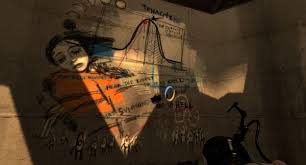
\includegraphics[width=0.6\textwidth]{chapters/15/images/Portal.png}
    \caption{Eine Grafik von dem beschrieben Portal Grafitti}
    \label{UST-6}
\end{figure}
Im Gegensatz zu environmental Stortelling darf das indexcial Storytelling mit dem Spieler agieren. Das bedeutet, dass das Spiel ihm helfen kann weiter zukommen in dem es den Spieler Tipps gibt. Die Steuerung kann auch durch ein Tutorial im Spiel erklärt werden.Aber auch durch Schilder oder Bücher die im Spiel verteilt sind können Storyinhalte besitzen.Ein gutes Beispiel wäre Super Mario 64 in dem der Spieler am Anfang ein Schild sieht, worin die Story als auch die Spielsteuerung erklährt wird. Wichtig ist, bei der Methode das es nicht das Spielerlebnis durch zu viele Interaktionen mit dem Spieler verschlechtert. 

\subsection{Spannung einer Handlung}
Die Handlung eines Spiel sollte immer spannend gehalten werden. Aber der den Spieler nie überfordern. Wenn der Spieler überfordert ist, ist dieser genervt und wie vielleicht nicht mehr das Spiel spielen. Aber die Story sollte auch nicht zu langweilig sein um das Spielerlebnis zu trüben. Zudem sollte die Handlung eines Spiel wie einen Film gleichen. Damit ist gemeint, das es am Anfang einen Aufbau der Story gibt. Danach bleibt die Steigung anhaltend bis am Schluss wo jeder Plot aufgelöst wird. Dieses verfahren wird in fast jeden literarischen Werk verwendet, ob es Film, ein Buch oder sogar ein Theater Stück. Dieses Schema ist beliebt da es Spannung erzeugt und den Endverbraucher (Spieler, Leser, Zuschauer) and die Geschichte klammert. 

\subsection{Spannung Gameplay}
Auch das Gameplay\footnote[1]{Gameplay ist wie sich das Spiel spielt.} muss eine gewisse Spannung habung. Wenn das Spiel zu leicht ist fühlt sich der Spieler unterfordert. Aber wenn das Spiel zu schwer ist er frustriert.\\\\
Wichtig ist das der Flow\footnote[2]{Spielefluss} optimal zum Spiel passt. Gehen davon aus es ist ein Spiel für jüngere verbraucher dann darf das Spiel nicht zu schwer sein da die Erfahrung mit Spielen einfach zu wenig vorhanden ist. Aber wenn Zielgruppe Personen sind die sich mit Videospielen gut auskennen, dann sollten sie auch Herausgefordert werden. Damit sie nicht während des Spielens aufgrund des zu leichten Gameplay keine lust mehr bekommen das Spiel zu spielen. Wichtig ist aber, dass der Flow während des Spielverlaufs ändert. Am Anfang sollte das Spiel einfach gehalten sein. Damit der User einen leichten Start in das Spiel bekommt. Wenn sich der Spieler an die Gamemechaniken\footnote[3]{Gamemechaniken sind Spielelemente welche man benötigt um das Spiel zu verwenden zum Beispiel Steurung und Fähigkeiten} gewöhnt hat, muss der Spieler mehr gefordert werden damit sein Interesse bleibt. Zudem fuhlt sich das Spiel eintönig and wenn immer die gleiche Herausforderung entgegen kommt. In der folgenden Abbildung aus dem Buch \citetitle{GameDesign} kann man erkennen der Flow sich während des Spiels veränder soll.

\begin{figure}[H]
    \centering
    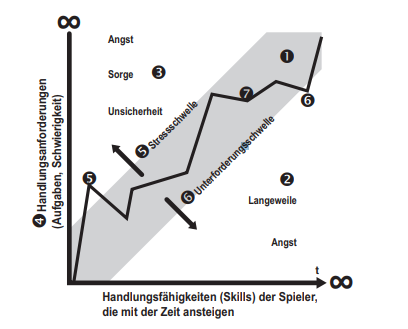
\includegraphics[width=0.8\textwidth]{chapters/15/images/GameFlow.png}
    \caption{Eine Grafik die den Flow verlauf des Spiels zeigt}
    \label{UST-4}
\end{figure}


\subsection{Theme}
Das Theme ist dafür zuständig um die visuellen und audiodiven Reize des Spielers zu begeistern. Eine gute Story macht es nicht automatisch zu einem guten Spiel. Das Theme muss zur Story passen. In einem fröhlichen Spiel sind die Farben meist bunt und die Hintergrund-Musik sehr fröhlich und aufmundert. Nicht wie bei einer düsteren beziehungsweise trarigen Story, da werden ehe dunklere Farben und eine langsame umklammertende Musik verwendet. Das Theme muss den Spieler stimmig für die Story machen.

\subsection{Spielidee für den Prototypen}
Für den Prototypen habe wir (Martin Usta und Lukas Schachinger) uns entschieden das wir einen Platformer\footnote[6]{Platformer ist ein Spielkonzept wo die Spielfigur auf Platformen spring um weiter zu kommen} machen. Dieser Sollte beinhalten Sammelobjekte in Form von Münzen. Aber auch schwierige Passage wo der Spieler sich gefordert fühlt. Der Spielbare Charakter sollte aufjeden fall dynamische Animationen besitzen. Zudem sollten auch Gegner in diesem Spiel vorkommen um den Spieler zuhindern das Ende zu erreichen. Die Inspiration für diese Art vom Spiel, war das damalige Kult Spiel "Kao the Kangaro Round 2" welches im Jahr 2004 im November erschiene ist.\\\\

\subsection{Storyline für den Prototypen}
Unser Hautprotagonist "generischer Name" ist eingeschlaffen und findet sich in eine Traumwelt als Eule wieder. Dieser versucht alles um dieser Welt zu entkommen. Doch diese Aufgabe ist schwieriger als er es vermuten mag. Um dieses Ziel zu beweltigen muss dieser Fallen ausweichen, Rätsel lösen und Gegener die ihm in den Weg stellen ausschalten. Dafür setzt er seine Eulenfähigkeiten ein. Ob in das gelingen wird ist nur eine Frage der Zeit. Aber er weiß er muss so schnell wie möglich aufstehen um sein Kind vom Kindergarten abzuholen. 


\begin{figure}[H]
    \centering
    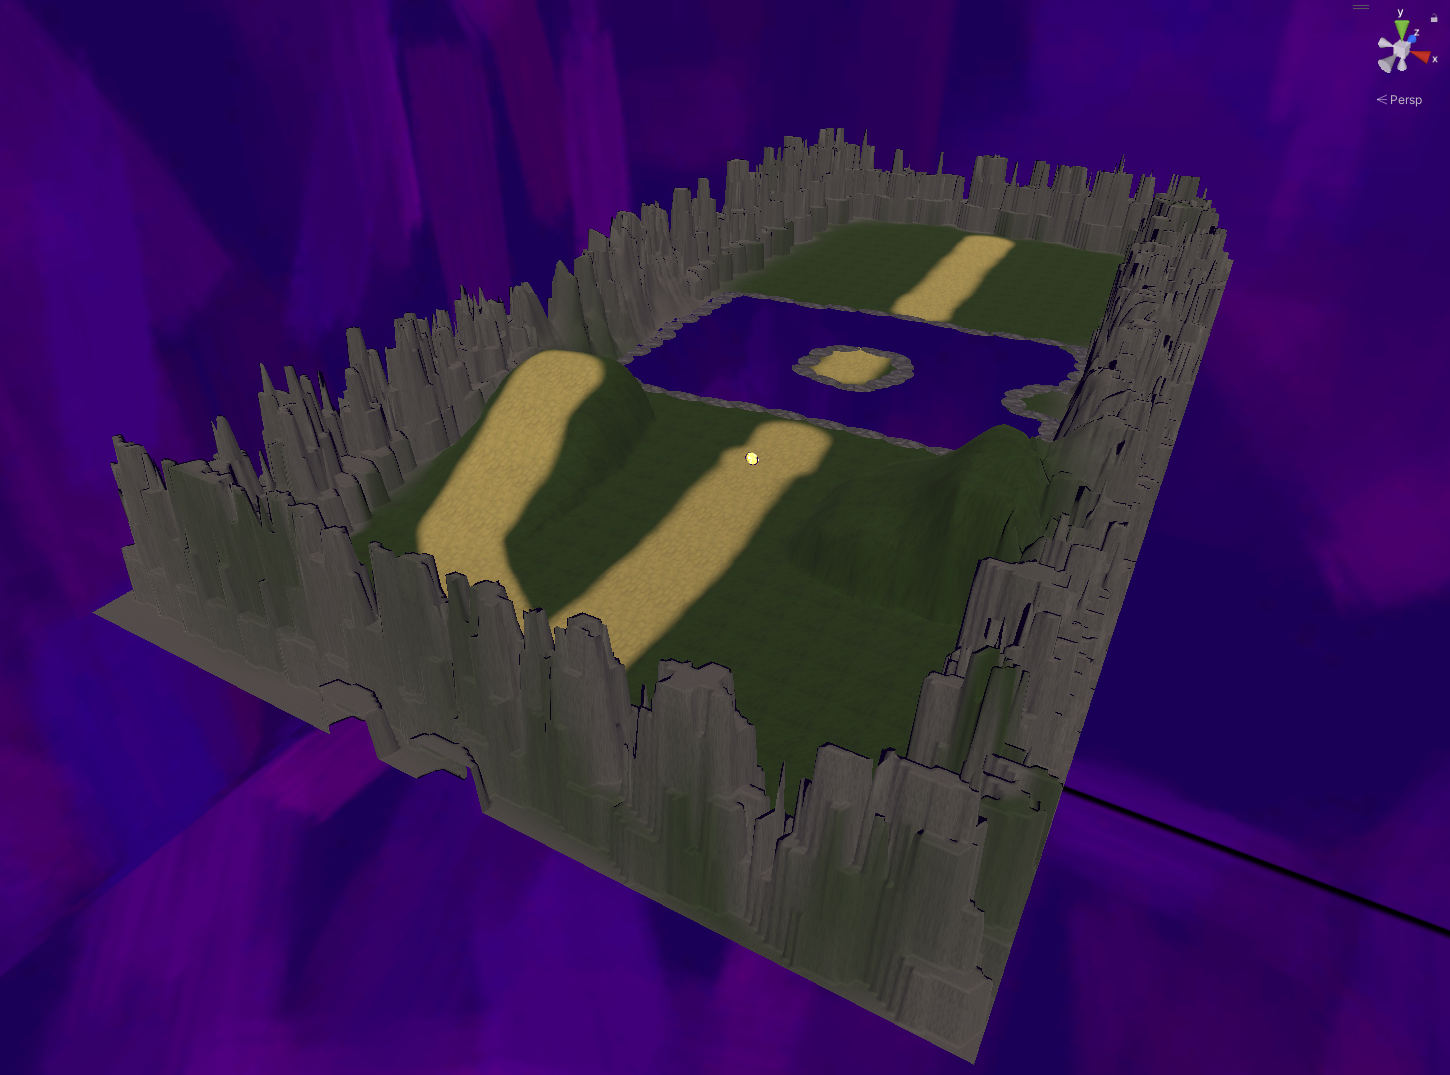
\includegraphics[width=0.8\textwidth]{chapters/15/images/Dreamworld.png}
    \caption{Eine Grafik des ersten Konzepts unsere Traumwelt}
    \label{UST-7}
\end{figure}

